\begin{figure}[t]
        \centering
	\begin{subfigure}[b]{0.45\textwidth}
	\begin{lstlisting}
	type Effect  String 
	type State = String 

	read :: State -> (String, Maybe Effect)
	read s = (s,Nothing)

	write :: String -> ((), Maybe Effect)
	write comment = ((), comment)

	apply :: State -> Effect -> State 
	apply s eff = in s ++ " - " ++ comment
	\end{lstlisting}
	\caption{Implementation}
	\label{subfig:comment_code}
	\end{subfigure}
	\hfill
	\begin{subfigure}[b]{0.49\textwidth}
	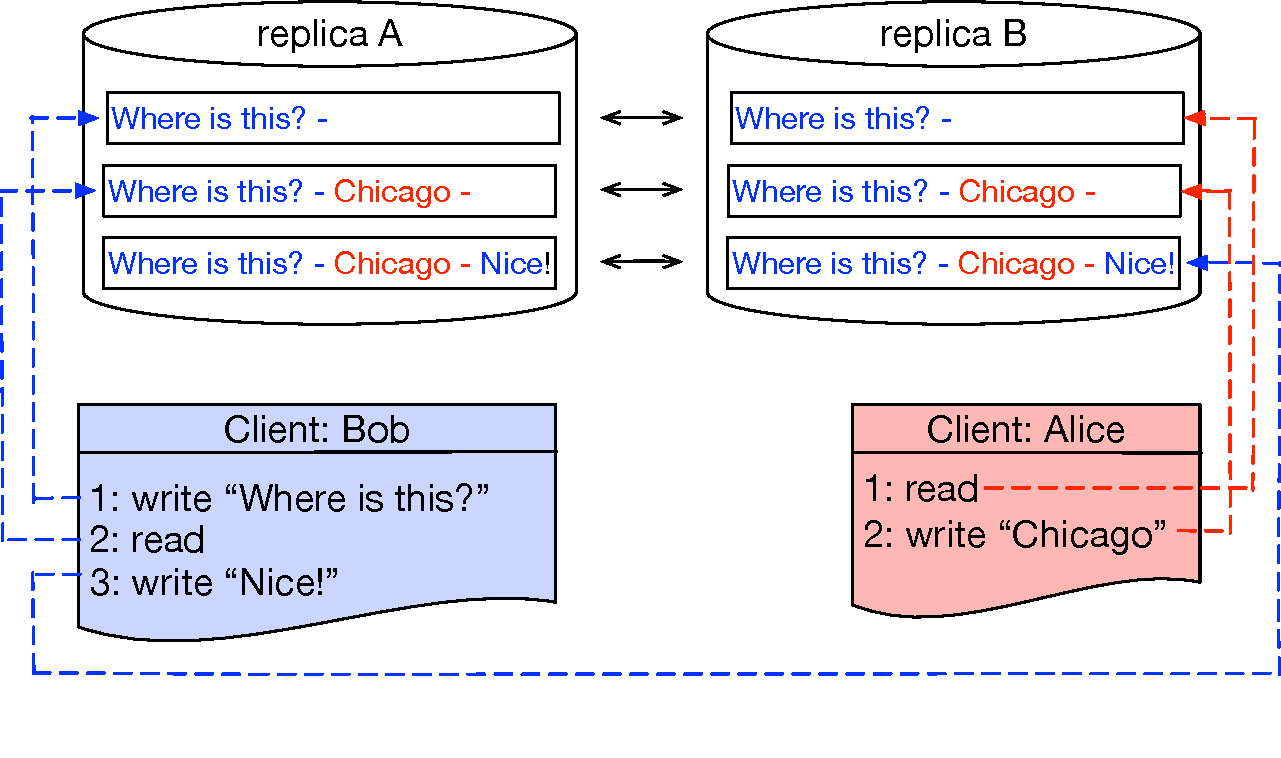
\includegraphics[scale=0.36]{Figures/comment_application.pdf}
	\caption{Example}
	\label{subfig:comment_example}
	\end{subfigure} 
\\ \hrulefill
\caption{A distributed application for comment section
management}
\label{fig:comment_app}
\end{figure}


